\section{Analysis}

Beyond performance, we analyze \emph{why} \ours{} works, focusing on design choices, evolution of curator's behaviors and contents in \textsc{SkillRepo}, and the role of curated skills in task success. Additional analyses are included in Appendix~\ref{app: additional_analysis}.


\begin{wraptable}{t}{0.36\textwidth}
% \vspace{-3mm}
\centering\setlength{\tabcolsep}{4.5pt}
\small
\setlength{\belowcaptionskip}{5pt}
  \caption{Ablation results of reward design on the ALFWorld dataset.}
  \label{table: ablation}
  \begin{tabular}{lcc}
    \toprule
   \textbf{Methods} &Avg. SR&Steps \\
    \midrule
    \ours-GRPO&61.2&18.9 \\
    \quad w/o $r^{cnt}$&58.6&20.1\\
    \quad w/o $r^{comp}$&60.0&19.3\\
    % \quad w/o both&&\\
    \hdashline
    \quad w/o grouping &57.3&20.6\\
  \bottomrule
\end{tabular}
\vspace{-5mm}
\end{wraptable}

\vspace{-3mm}
\paragraph{Ablation Studies.}
We ablate two components of \ours{}: (i) auxiliary rewards in Eq.~\ref{eq:reward}, and (ii) grouped task streams in \S~\ref{sec:training_instance_construction}. Experiments are conducted on ALFWorld, with Qwen3-8B used as both the curator and executor. As shown in Table~\ref{table: ablation}, removing either reward component hurts performance. Without the content-quality reward, the success rate drops from 61.2 to 58.6, showing the importance of intermediate supervision for guiding skill updates in a pipelined system. Removing the compression reward causes a smaller but consistent drop, suggesting that concise repositories are easier for the executor to use. The most significant degradation comes from using random task sequences (w/o grouping), which lowers the success rate to 57.3. This highlights the importance of training on grouped task streams, in which curation decisions are learned from their downstream impact on related future tasks.


\begin{wrapfigure}{r}{0.4\textwidth}
\vspace{-3mm}
  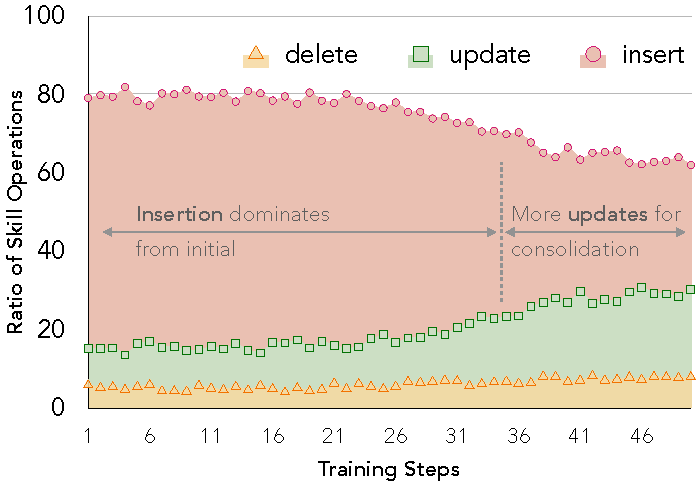
\includegraphics[width=0.4\textwidth]{figures/ops_ratio.pdf}
  \vspace{-5mm}
  \caption{Behaviors of the skill curator w.r.t. skill operations during training.}
  \label{fig: skill-ratio}
  \vspace{-5mm}
\end{wrapfigure}
\noindent\textbf{Behaviors of Skill Curator.}
To better understand how the behavior of the skill curator evolves during training, we analyze the distribution of its three skill operations from rollouts at different training steps: \insertop, \updateop, and \deleteop. Figure~\ref{fig: skill-ratio} plots the proportion of each operation.
At the beginning of training, \texttt{insert} overwhelmingly dominates, indicating that the model is primarily focused on populating the skill repository with new knowledge distilled from experience. As training progresses, however, \texttt{update} becomes increasingly frequent, while \texttt{insert} steadily declines. This suggests that the skill curator gradually moves from plain expansion of skills to refining existing skills. Meanwhile, \texttt{delete} remains a relatively small fraction throughout training with a slightly growing trend, showing the effectiveness of rewarding conciseness of \textsc{SkillRepo}. Instead, the dominant form of adaptation is to revise and consolidate previously acquired skills.

\begin{figure}[H]
\begin{center}
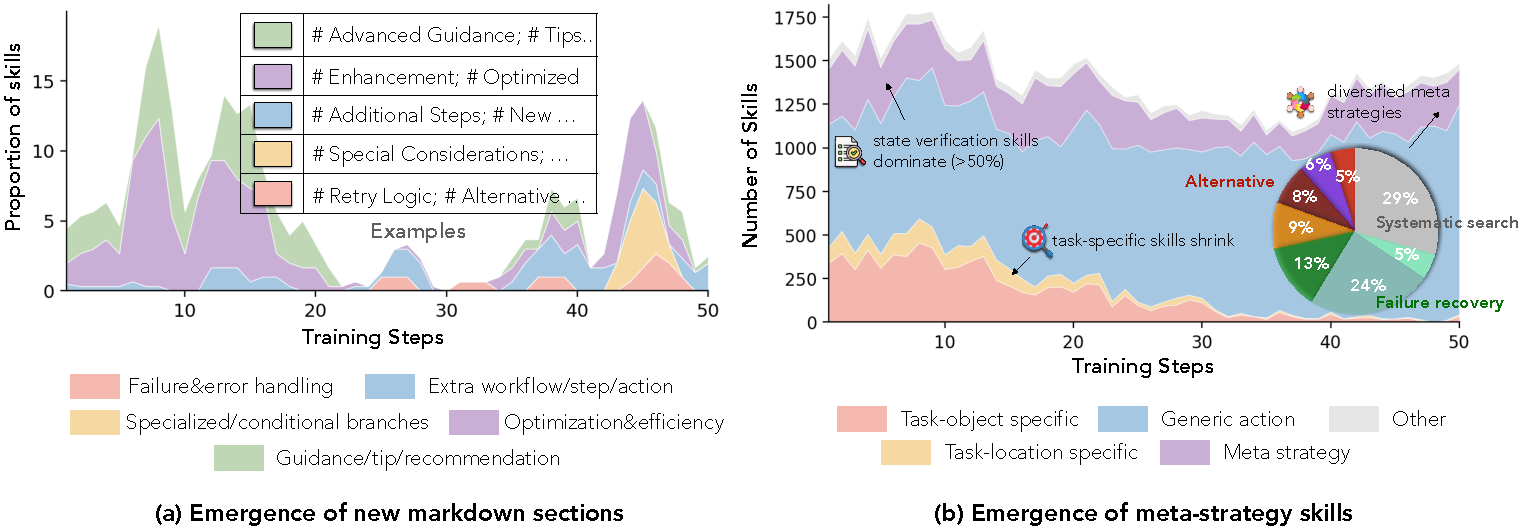
\includegraphics[width=\textwidth]{figures/skill_evol.pdf}
\end{center}
\vspace{-3mm}
\caption{Evolution dynamics of the curated skills under RL training.}
\label{fig: skill_evol}
\vspace{-5mm}
\end{figure}

\noindent\textbf{Skill Evolution Dynamics.}
Beyond aggregate performance, we examine how the skill repository evolves during RL training. 
We focus on two emergent phenomena: (i) new Markdown sections within individual skills, and (ii) higher-level meta-skills that capture reusable principles across tasks. 
Figure~\ref{fig: skill_evol}(a) shows that early in training, the curator tends to introduce generic sections such as additional guidance, tips, or recommendations, which often make skills more verbose without substantially improving their operational value. 
As training progresses, these additions shift toward more actionable structures, such as failure-handling logic and conditional branches that specify when to deviate from the default workflow. 
This suggests that RL gradually steers the curator from superficial enrichment toward execution-oriented skill refinement.
Figure~\ref{fig: skill_evol}(b) further shows that evolution occurs not only within individual skills, but also in the global organization of the repository. 
Early repositories are dominated by narrow, task-specific skills, whereas later repositories contain a more diverse set of meta-strategy skills covering verification, fallback planning, system search, and strategy adjustment. 
This indicates that the learned curator does not merely accumulate skills, but progressively expands the repository's strategic space, shifting it from isolated task-local procedures toward more compositional cross-task control knowledge.



\begin{wrapfigure}{r}{0.4\textwidth}
\vspace{-3mm}
  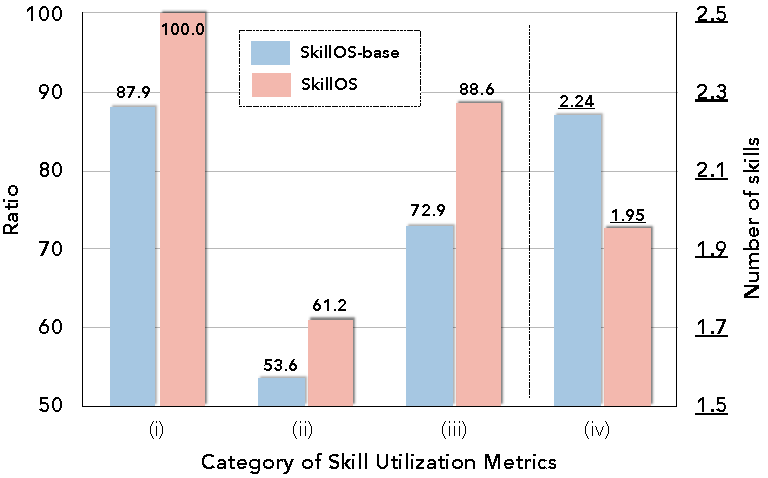
\includegraphics[width=0.4\textwidth]{figures/skill-usage.pdf}
  \vspace{-5mm}
  \caption{Comparison of skill utilization statistics on ALFWorld.}
  \label{fig: skill-usage}
  \vspace{-5mm}
\end{wrapfigure}

\noindent\textbf{Attribution of Skill Usage.}
To better understand whether the gains of \ours{} come from the evolved skills, we analyze how skills are used during evaluation. 
We consider 4 complementary metrics: (i) \emph{skill usage rate}, the fraction of examples where the agent invokes at least one skill; (ii) \emph{successful skill usage rate}, the success rate among examples that use skills; (iii) \emph{skill coverage}, the fraction of the skill collection that are actually used; and (iv) the \emph{average number of skills used per example}, which measures the degree of skill reliance.
Figure~\ref{fig: skill-usage} reports results on ALFWorld. 
Compared with the baseline, \ours{} invokes skills on \emph{all} evaluation examples and achieves a higher success rate, indicating that the evolved skills contribute directly to task solving. 
Also, a larger fraction of the skill curated by \ours{} is used, showing that RL training improves the overall utility of the curated \textsc{SkillRepo}.
Meanwhile, \ours{} uses fewer skills per example, suggesting that gains come from more precise skill selection rather than more skill context.